\section{Entwicklungsumgebung Eclipse}

Eclipse ist eine freie Entwicklungsumgebung welche ursrp�nglich f�r die Sprache Java entwickelt wurde. Mittlerweile gibt es Eclipse Plug-ins f�r weitere Programmiersprachen wie C, C++ oder Pearl.
Wie die meisten Entwicklungsumgebungen bietet Eclipse eine Vielzahl, dem Entwickler n�tzlicher, Funktionen. Dazu geh�ren das Debuggen des Programmcodes, automatische Erstellen von Get- und Set- Methoden sowie automatische Codevervollst�ndigung. �ber automatische Kontexthilfe liefert Eclipse Vorschl�ge um Fehler zu beheben.
Eclipse kann leicht durch den Eclipse Marketplace mit verschienden Plug-Ins erweitert werden. F�r die Verbindung von Eclipse mit dem eingesetzten Versionsverwaltungs System Git wurde das Plug-In EGit verwendet.


\begin{figure}[h]
\centering
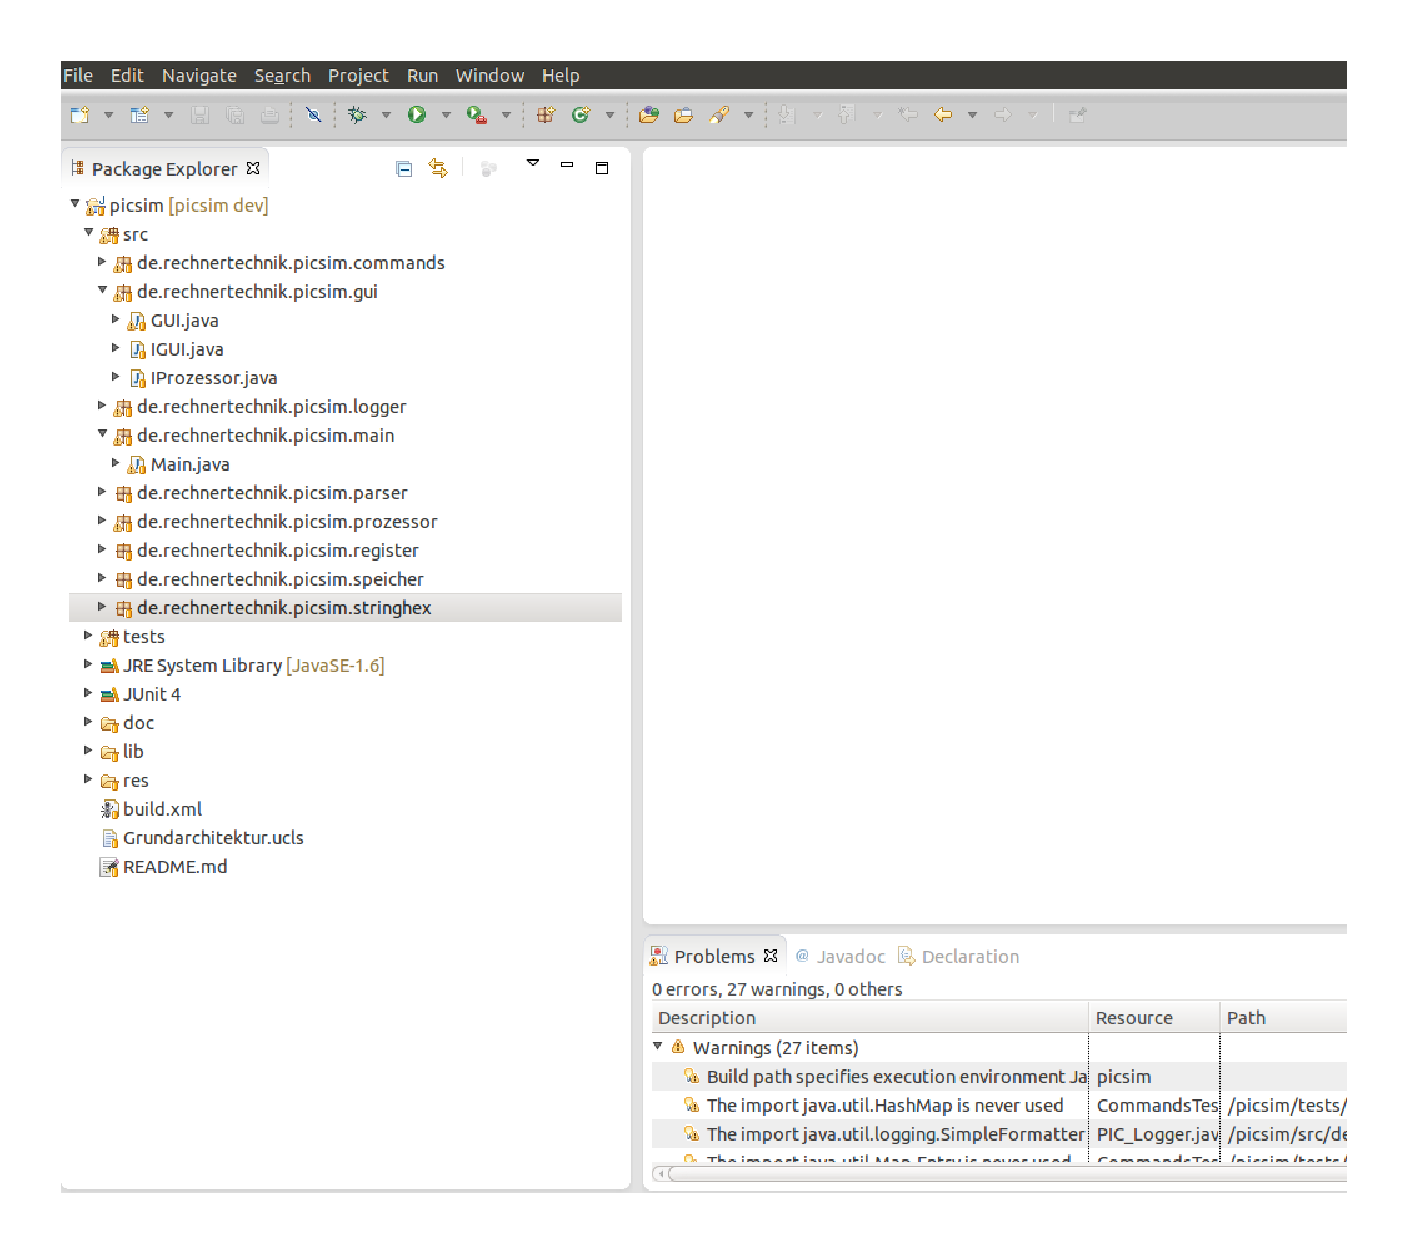
\includegraphics[scale=0.25]{Bilder/Eclipse.pdf}
\caption{Eclipse}
\end{figure}